
\vspace{-5mm}
This chapter gives routines for computing translation matrices that operate on the spherical wave function expansions given in Chapter \ref{chap:wavefunctions}. Translation matrices, which are derived from addition theorems, allow us to represent a scalar or vector field in two different but parallel reference frames. The frame of reference is being translated, not the field. The addition theorems and matrix diagonalization are first outlined. Next, algorithms and routines for the scalar axial translation matrices (i.e., translation along the $z$-axis) are given which are computed on full or sparse matrices. Last, algorithms and routines for full and sparse vector axial translation matrices are derived from the scalar versions.  

\vspace{-2mm}
\section{Translation Addition Theorem}

The translation addition theorems for spherical wave functions allow the same field to be expanded in two different, but parallel, frames. These are given for scalar waves as \cite{chew1995waves}, 
\begin{eqnarray}
\psi_{l'm'}(k,\br_i) &=& \sum_{l=0}^{\infty}\sum_{m=-l}^{l} \alpha^{ji}_{lm,l'm'} \textit{Rg}\psi_{lm}(k,\br_j), \quad \quad r_j < r_{ji} \label{adthmscal1} \\
\psi_{l'm'}(k,\br_i) &=& \sum_{l=0}^{\infty}\sum_{m=-l}^{l} \beta^{ji}_{lm,l'm'}\psi_{lm}(k,\br_j), \quad \quad r_j > r_{ji} \label{adthmscal2}\\
\textit{Rg}\psi_{l'm'}(k,\br_i) &=& \sum_{l=0}^{\infty}\sum_{m=-l}^{l} \beta^{ji}_{lm,l'm'}\textit{Rg}\psi_{lm}(k,\br_j), \quad \quad \forall r_j \label{adthmscal3}  
\end{eqnarray}

\noindent where $\beta^{ji}_{lm,l'm'} = \textit{Rg} \alpha^{ji}_{lm,l'm'}$ are translation matrices and $\textit{Rg}$ is the regular part. The position vectors, $\br_i$ and $\br_j$, are measured from the origins of each frame. The first relation expands radiating waves from frame $i$ as regular or incoming waves in frame $j$. The second expands radiating waves in frame $i$ as radiating waves in frame $j$. The last expresses regular waves in frame $i$ and regular waves in frame $j$. Each addition theorem has a different region of validity: \eqref{adthmscal1} is valid within a sphere of radius $r_{ji} = \vert \bb{r}_{ji} \vert = \vert \br_j- \br_i\vert$ centered on frame $j$; \eqref{adthmscal2} is valid outside a radius $r_{ji}$ centered on frame $j$; \eqref{adthmscal3}  is valid everywhere. 

Translation addition theorems for vector spherical wave functions have similar structures, \cite{chew1995waves}. The first is 
\begin{eqnarray}
\bb{M}_{l'm'}(k,\br_i) &=& \sum_{l=1}^{\infty}\sum_{m=-l}^{l} A^{ji}_{lm,l'm'} \textit{Rg}\bb{M}_{lm}(k,\br_j),  + B^{ji}_{lm,l'm'} \textit{Rg}\bb{N}_{lm}(\br_j) \\
\bb{N}_{l'm'}(k,\br_i) &=& \sum_{l=1}^{\infty}\sum_{m=-l}^{l} B^{ji}_{lm,l'm'} \textit{Rg}\bb{M}_{lm}(k,\br_j),  + A^{ji}_{lm,l'm'} \textit{Rg}\bb{N}_{lm}(\br_j)
\end{eqnarray}

\noindent where $A^{ji}_{lm,l'm'}$ and $B^{ji}_{lm,l'm'}$ are vector translation matrices and is valid for $r_j < r_{ji}$. The remaining two relations are analogous to the scalar case and can be obtained with appropriate Hankel or Bessel functions in $A^{ji}_{lm,l'm'}$ and $B^{ji}_{lm,l'm'}$. These show that vector modes mix when translated. The spherical vector components are also transformed and are expressed relative to the origin of the new frame. This means that the vector components in each frame need to be converted to Cartesian components before comparing.


\begin{figure}[H] 
   \centering
   \includegraphics[width=3.5in]{Translation/Figures/transdiagram} 
   \caption{Coordinate frames $i$ and $j$.}
   \label{translationadd}
\end{figure}


Translation matrices allow us to manipulate field using only the expansion coefficients.  For example, a radiating scalar field is expanded in frame $i$ as 
\begin{equation}
\phi(\br_i) = \sum_{l'=0}^{\infty}\sum_{m'=-l'}^{l'} a_{l'm'} \psi_{l'm'}(\br_i)
\end{equation}

The same field expressed as incoming waves in frame $j$ comes from substituting \eqref{adthmscal1} and regrouping terms as
\begin{eqnarray}
\phi(\br_j) &=& \sum_{l=0}^{\infty}\sum_{m=-l}^{l} b_{lm}  \textit{Rg}\psi_{lm}(k,\br_j) \\
b_{lm} &=& \sum_{l'=0}^{\infty}\sum_{m'=-l'}^{l'} \alpha^{ji}_{lm,l'm'}a_{l'm'}
\end{eqnarray}
%
%\begin{eqnarray}
%\phi(\br_j) &=& \sum_{l'=0}^{\infty}\sum_{m'=-l'}^{l'} a_{l'm'} \sum_{l=0}^{\infty}\sum_{m=-l}^{l} \alpha^{ji}_{lm,l'm'} \textit{Rg}\psi_{lm}(k,\br_j) \nonumber \\
%\ &=& \sum_{l=0}^{\infty}\sum_{m=-l}^{l} b_{lm}  \textit{Rg}\psi_{lm}(k,\br_j) \\
%b_{lm} &=& \sum_{l'=0}^{\infty}\sum_{m'=-l'}^{l'} \alpha^{ji}_{lm,l'm'}a_{l'm'}
%\end{eqnarray}

Likewise, for the other relations. In matrix notation this is 
\begin{eqnarray}
\phi(k,\br_i) &=&  \boldsymbol{\psi}^t(k,\br_i)\cdot \bb{a} \\
\phi(k,\br_j) &=&  \textit{Rg}\boldsymbol{\psi}^t(k,\br_j)\cdot \bb{b} \\
\bb{b} &=& \boldsymbol{\alpha}_{ji} \bb{a}
\end{eqnarray}

The analogous matrix notation for vector waves is
\begin{eqnarray}
\bb{E}(k,\br_i) &=& \rvectwo{\bb{M}^t(k,\br_i)}{\bb{N}^t(k,\br_i)}\cvectwo{\bb{a}}{\bb{b}} \\
\bb{E}(k,\br_j)&=& \rvectwo{\Re\bb{M}^t(k,\br_j)}{\Re\bb{N}^t(k,\br_j)}\cvectwo{\bb{c}}{\bb{d}} \\
\cvectwo{\bb{c}}{\bb{d}}  &=&\tbt{\bb{A}_{ji}}{\bb{B}_{ji}}{\bb{B}_{ji}}{\bb{A}_{ji}}\cvectwo{\bb{a}}{\bb{b}}
\end{eqnarray}

In both scalar and vector cases the transpose, $^t$, means align the harmonic indices along columns. Technically the sums are infinite, but the matrices are always truncated in practice.

\section{Diagonalization}

Explicit expressions for the matrix elements of the scalar and vector translation matrices are given in \cite{chew1995waves}, but are given in terms of Wiger 3-j symbols, which are slow and inaccurate to compute. Fast recursions for quickly computing the scalar and vector translation matrices were developed in \cite{mackowski1991analysis, chew1992recurrence, chew1993efficient}.  

The standard way to compute the translation matrix is to break it into three matrices. The local frame, $i$, is first rotated to point its $z$-axis toward the destination frame, $j$. The local frame is then axially translated. Finally, the frame is then rotated back. This effectively diagonalizes the translation matrix. Specifically, if the vector $\br_{ji}$ points from the origin of frame $i$ to the origin of frame $j$, with magnitude $r_{ji}$ and spherical angles $\theta_{ji}$, $\phi_{ji}$, shown in Figure \ref{translationadd}, then the scalar translation matrix is expanded (diagonalized) as
\begin{equation}
\boldsymbol{\alpha}_{ji} = \bb{D}^*(\phi_{ji}+\pi/2,\theta_{ji},0) \cdot \boldsymbol{\alpha}_z(r_{ji}) \cdot \bb{D}(\phi_{ji}+\pi/2,\theta_{ji},0)
\label{alphazdiag}
\end{equation}

\noindent where $\bb{D}$ is the rotation matrix with ZXZ convention, and $\boldsymbol{\alpha}_z(r_{ji})$ is the axial translation matrix in the $+z$ direction. The factor of $\pi/2$ ensures that $\theta_{ji}$ tips the $z$-axis toward the destination frame with a right-handed X rotation. The sequence starts with an inverse rotation on the right size because we first view the field, which is fixed in the global frame, from the point of view of the rotated frame. Next, this point of view is translated along the $z$-axis of the rotated frame. Finally, the reverse rotation (in this case a forward rotation) is applied to bring the frame back to be parallel with the global frame. This procedure also applies to the vector translation matrices $\bb{A}_{ji}$ and $\bb{B}_{ji}$.  

\begin{figure}[H] 
   \centering
   \includegraphics[width=5in]{Translation/Figures/alphaz} 
   \caption{Diagonalization of the scalar translation matrix.  L = 6.  Left is the full translation matrix.  Right shows the two rotation matrices bookending the z-axial translation matrix.}
   \label{figdiag}
\end{figure}


While one can reduce the recurrence relations for the full translation matrices given in \cite{chew1992recurrence, chew1993efficient} to the axial case, equations for the axial scalar translation are derived directly in \cite{mackowski1991analysis}, from which the axial vector translations follow. These are given succinctly in \cite{duan2015experimental}.  

The reason for the dramatic speed up of the matrix-vector multiplication in the case of diagonalization over the full matrix is because the rotation matrix is block diagonal and the $z$-axial translation requires the fewest non-zero terms of all possible translation directions. Together these yield many fewer overall multiplications than when using the full matrix, and the computational advantage grows as the matrix grows. In addition, the rotation matrix only needs to be computed once (the inverse is just conjugate). If the translation matrix is non-square, as will be the case when the number of harmonics between two frames is different, then the rotation matrix can be computed once for the larger of $L$ and $L'$, which are the largest degree along row and column, respectively, and then truncated.  Figure \ref{figdiag} illustrates the diagonalization of the translation matrix. The matrices must be applied individually to the expansion coefficients from right to left, otherwise the benefits of diagonalization are lost.


%[10] W. C. Chew, ?Recurrence Relations for Three-Dimensional Scalar Addi- tion Theorem?, Journal of Electromagnetic Waves and Applications, Vol. 6, No. 2, pp. 133-142, 1992.
%[11] Daniel W. Mackowski, ?Analysis of Radiative Scattering for Multiple Sphere Configurations?, Proceedings: Mathematical and Physical Sciences, Vol. 433, No. 1889, pp. 599-614, Jun. 1991.

\clearpage
\newpage
\section{Scalar Translation Matrix}

In this section we give a routine for the scalar axial translation matrix. We then derive a routine for indexing and computing the inherently sparse scalar axial translation matrix on a 1D array. We also give a routine that accomplishes the diagonalized matrix-vector multiplication and operates on the expansion coefficients directly. Finally, we provide a routine that computes the full scalar translation matrix directly. 

\subsection{Scalar Axial Translation Matrix}

The recurrence equations for the scalar axial translation matrix, \eqref{alphazdiag}, follow \cite{mackowski1991analysis}.  The matrix elements are zero except for $m = m'$.  Let $(l,m)$ and $(l',m')$ correspond to the rows and columns, respectively.  While the sums are technically infinite, they are always truncated at maximum orders $L$ and $L'$, respectively.

The calculation is initialized with 
\begin{equation}
\alpha_{l,0,0,0} = (-1)^l\sqrt{2l+1}h_l^{(1)}(kr_{ji})
\end{equation}

Next, $\alpha_{l,m,l',\vert l'\vert}$ is computed from 
\eq{\alpha_{l,l'+1, l'+1,l'+1} = \sqrt{\dfrac{2l'+3}{2(l'+1)}} \left[\sqrt{\dfrac{(l+l'+1)(l+l')}{(2l-1)(2l+1)}} \alpha_{l-1,l',l',l'}  +   \sqrt{\dfrac{(l-l'+1)(l-l')}{(2l+3)(2l+1)}} \alpha_{l+1,l',l',l'}    \right]
}

%\begin{eqnarray}
%\alpha_{l,l'+1, l'+1,l'+1} &=& \sqrt{\dfrac{2l'+3}{2(l'+1)}} \left[\sqrt{\dfrac{(l+l'+1)(l+l')}{(2l-1)(2l+1)}} \alpha_{l-1,l',l'l'} \right. \nonumber \\
%\ & \ & \left. +   \sqrt{\dfrac{(l-l'+1)(l-l')}{(2l+3)(2l+1)}} \alpha_{l+1,l',l'l'}    \right]
%\end{eqnarray}

and $\alpha_{l,-l', l',-l'} = \alpha_{l,l',l',l'}$.  The remaining coefficients are obtained for $m = \pm l'$ using
\eq{\alpha_{l,m,l'+1,m} = \sqrt{2l'+3}\left[\sqrt{\dfrac{(l+l')(l-l')}{(2l-1)(2l+1)}} \alpha_{l-1,m,l',m}  -  \sqrt{\dfrac{(l+l'+1)(l-l'+1)}{(2l+3)(2l+1)}} \alpha_{l+1,m,l',m}    \right] 
}

%
%\begin{eqnarray}
%\alpha_{lm,l'+1,m} &=& \sqrt{2l'+3}\left[\sqrt{\dfrac{(l+l')(l-l')}{(2l-1)(2l+1)}} \alpha_{l-1,m,l'm}  \right.\nonumber \\
%\ & \ & - \left.  \sqrt{\dfrac{(l+l'+1)(l-l'+1)}{(2l+3)(2l+1)}} \alpha_{l+1,m,l'm}    \right] \nonumber \\
%\end{eqnarray}

and $m \ne \pm l'$ using
\begin{eqnarray}
\alpha_{l,m,l'+1,m} &=& \sqrt{\dfrac{(2l'+3)(2l'+1)}{(l'+m+1)(l'-m+1)}}\left[  \sqrt{\dfrac{(l'+m)(l'-m)}{(2l'+1)(2l'-1)}} \alpha_{l,m,l'-1,m}   \right. \nonumber \\
\ & \ & \left. + \sqrt{\dfrac{(l+m)(l-m)}{(2l+1)(2l-1)}}\alpha_{l-1,m,l',m} - \sqrt{\dfrac{(l+m+1)(l-m+1)}{(2l+3)(2l+1)}}\alpha_{l+1,m,l',m} \right] \nonumber \\
\end{eqnarray}

That's about as confusing as it gets.  Some comments on computation:

\begin{enumerate}
\item The equations in \cite{mackowski1991analysis} allow for translation in $\pm z$ directions.  We only translate in $+z$.  

\item The algorithm iterates on $l+1$ for an element at $l'+1$. This has a cascading effect that, in order to compute the lower right block at $l = L$ and $l' = L'$, an additional element at $L+1$ is required, and so on.  For example, if the translation matrix is square, we must fill a triangular region to $l = L + L'$ at $l'=0$.  This is explained in detail in \cite{chew1992recurrence}.  Once the computation is finished, the matrix is cropped to the intended size.  

\item We need to accommodate non-square matrices for translation of expansions of different harmonic content.  Because of the filling requirement above, it is advantageous to create the fill region in the direction of the larger of $L$ and $L'$.  Rather than rewrite the routine to fill along rows or columns, we can make use of the follow transpose relation 
\begin{equation}
\alpha^{ij}_{lm,l'm'} = (-1)^{l+l'}\alpha^{ji}_{lm,l'm'} \label{azflip}
\end{equation}

The triangular fill region is appended to the bottom of the matrix, along the rows up to $\textrm{max}(L,L')$. The matrix is then cropped and transposed if $L' > L$.  

\item The computation is the same for $\alpha$ or $\beta$, only the Bessel function changes at the initialization.  

\end{enumerate}


\begin{figure}[H] 
   \centering
   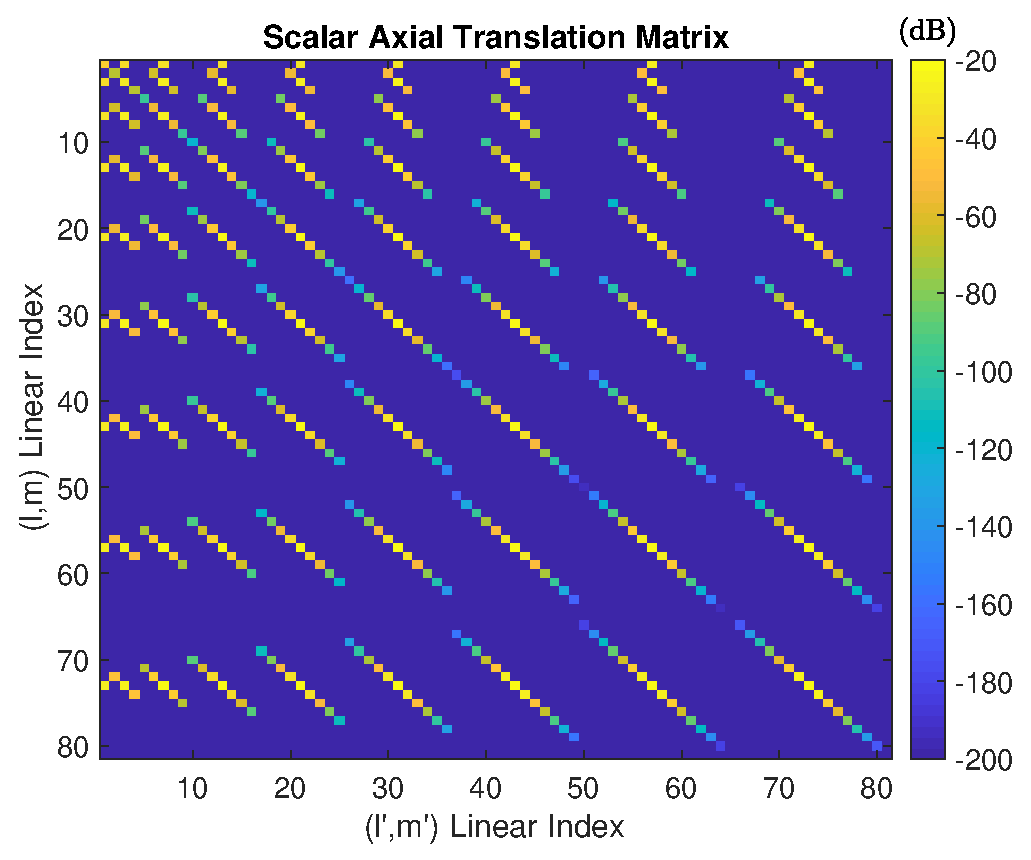
\includegraphics[width=3.5in]{Translation/Figures/trans1} 
   \caption{Scalar axial translation matrix, $L = L' = 8$, $k = 1$, $r_{ji} = 100$. }
   \label{fig4}
\end{figure}



The routine \texttt{alphaz} takes as input the largest row degree, $L$, the largest column degree $L'$, wavenumber $k$, axial translation distance $r_{ji}$, and returns the translation matrix in full, including zeros.  Use string switch \texttt{'rg'} for the regular form. This routine is a good starting point for visualization, but the output matrix should not be used as is for matrix-vector multiplication due to the zeros, or it should be converted to a sparse matrix. The routine is written with the variable $n$ in place of $l'$ for clarity. 

{\footnotesize
\VerbatimInput{\code/Translation/alphaz.m}
}


\clearpage
\subsection{Sparse Scalar Axial Translation Matrix}

We want to compute the inherently sparse axial translation matrix on a 1D array, to avoid preallocating a potentially massive, mostly zero, matrix. Indexing is more complicated than for the sparse rotation matrix due to different sized diagonal subblocks as well as the triangular fill region requirement. Analytic formulas for sparse indexing are derived and used below. As implemented, these add a little computation time relative to indexing on the full preallocated matrix. 

\begin{figure}[H] 
  \centering
 \includegraphics[width=5.5in]{Translation/Figures/sparseindex_2} 
   \caption{Indexing the diagonal subblocks of the sparse scalar axial translation matrix. Blue arrows indicate the direction of the linear indexing.  }
   \label{fig2translation}
\end{figure}


The total number of non-zero matrix elements in the scalar axial translation matrix, but not including the required triangular fill region, is counted as 
\begin{eqnarray}
N(L,L') &=& \sum_{l' = 0}^{L'} \sum_{l=0}^{L} \sum_{m = -\textrm{min}(l,l')}^{\textrm{min}(l,l')} 1 \label{eq:NLL}\\
\ & = & \sum_{l' = 0}^{L'} \sum_{l=0}^{L} \left( \textrm{2 min}(l,l') + 1 \right) \label{crazysparse}
\end{eqnarray}  

This counts the total number of elements in a matrix that has $L \times L'$ subblocks. The number of non-zero elements along the diagonal of a subblock is determined by the smaller of the $l$ and $l'$. See Figure \ref{fig2translation}.  Plugging \eqref{crazysparse} into Wolfram Alpha we get
\begin{equation}
N(L,L') 
= \left\{
\begin{array}{ccc}
1 & \ & L =  L' = 0 \\
L'+1 &\ & L = 0, L' >0\\
L + 1 & \ & L' = 0 , L>0\\
-L'^3/3+L'^2 L+L' (2 L+4/3)+L+1 & \ & L'<L, L>0,L'>0 \\
-L^3/3+L^2 L'+L (2 L'+4/3)+L'+1 & \ & L'>L, L>0,L'>0 \\
2/3L^3 + 2L^2 + 7/3L + 1 & \ & L' = L, L>0,L'>0 \\
\end{array}
\right.
 \label{eq:a1}
\end{equation}

Next, the total number of nonzero elements in the triangular fill region, see Figure \ref{fig2translation2}, assuming $L \ge L'$, and assuming that the original matrix is extend along rows, is given by 
\begin{equation}
N_{\textrm{fill}}(L,L') = \sum_{l' = 0}^{L'-1} \sum_{l=L+1}^{L + L' - l'} \left( 2 l' + 1 \right) = L'(2L'^2 + 3L' + 1)/6  \label{eq:a2}\end{equation}



\begin{figure}[H] 
   \centering
      \includegraphics[width=3.5in]{Translation/Figures/sparseindex_3} 
   \caption{Indexing the diagonal subblocks of the triangular fill region of the sparse scalar axial translation matrix. Blue arrows indicate the direction of the linear indexing. }
   \label{fig2translation2}
\end{figure}


Because we have defined the fill region as additional matrix rows, the 1D crop is easiest if we index the diagonal $(l,l')$ subblocks as "row"-major (left-right, top-down), and where we index the diagonals of the subblocks from upper left to lower right. See again Figure \ref{fig2translation}. Once the computation is complete we keep the first $N(L,L')$ elements and apply the transpose if $L' > L$.  

The "row"-major 1D linear index for the axial translation matrix, but not including the triangular fill region, is given by  
\begin{equation}
I(l,l',m,L') = N(l-1,L') + \sum_{i = 0}^{l'-1}  (2\textrm{min}(l,i) + 1)  + (\textrm{min}(l,l') + m + 1)   \label{eq:a3}
\end{equation}

\noindent where
\begin{equation}
\sum_{i = 0}^{l'-1}  (2\textrm{min}(l,i) + 1) = 
\left\{\begin{array}{cc} 
l'^2, & l' = 1 \lor ( l+1>l' \land l' > 1) \\
-l^2 - l + 2ll' + l' & \textrm{otherwise} \\
\end{array}
\right\}
\end{equation}  

$N(l-1,L')$ counts the submatrix containing all diagonal subblocks up to but not including the desired $l$ row of diagonal blocks. The second term counts completed column blocks in the current row block up that go up to but do not include the desired $l'$. The last term counts the desired diagonal. This counting requires knowledge of $L'$.

Finally, the linear index of an element in the triangular fill region under the conditions that $L \ge L'$, $l > L$, and $0 \le l' \le L'-1$ is
\begin{eqnarray}
I_{\textrm{fill}}(l,l',m,L,L') &=& N(L,L') + \sum_{i= L+1}^{l-1} \left(\sum_{j=0}^{L'-1-(i-L-1)}(2j+1)\right) \nonumber \\
\ & \ & + \left(\sum_{j=0}^{l'-1} (2j + 1)\right) + (l' + m + 1)  \label{eq:a4} \\
\ & =& N(L,L') + \left( 1/6(l-L-1)(2l^2-l(4L+6Lp+7)+2L^2\right. \nonumber \\
\ & \ & \left. +L(6Lp+7)+6(Lp+1)^2)\right) + l'^2 + (l' + m + 1) 
\end{eqnarray}

The first term counts the number of elements in the actual matrix.  The second term counts the completed row blocks up to but not including the current row block in the fill triangle.  The third term counts the column blocks in the current row block to go up to but do not include the active diagonal (this is made simpler by the fact that $l' < l$ in the fill region).  The last term indexes the active diagonal.  



The routine \texttt{alphazSparse} returns three column arrays of the row index, column index, and matrix entries of the sparse axial translation matrix.  It is the same as \texttt{alphaz} but computed and output on a 1D array. Helper functions are given in Table \ref{sparsetranshelp}. \texttt{Nalphaz} and \texttt{Nalphazfill} count the number of nonzero elements in the matrix and fill region, respectively. \texttt{indAlphazFill} is used to index the sparse matrix including the fill regions; it calls \texttt{indAlphaz} which indexes the primary sparse matrix.  When $L' > L$, the transpose is accomplished by applying \eqref{azflip} and reordering row, column, and array elements to be consistent with the row-major indexing of \texttt{indAlphaz}.  


\begin{table}[htbp]
\caption{\texttt{alphazSparse} Helper Functions}
\begin{center}
\begin{tabular}{|c|c|c|}
\hline
Routine & Equation & Description \\
\hline
\texttt{Nalphaz} &   \eqref{eq:a1} & Number of non-zero elements in $L \times L'$ sparse $\alpha_{lm,l'm'}$ \\
\hline
\texttt{Nalphazfill} &  \eqref{eq:a2} & Number of non-zero elements in fill region \\
\hline
\texttt{indAlphaz} &   \eqref{eq:a3} & Row-major 1D linear index in sparse $\alpha_{lm,l'm'}$ \\
\hline
\texttt{indAlphazFill} &  \eqref{eq:a4} & Row-major 1D linear index in sparse fill region \\ 
\hline
\end{tabular}
\end{center}
\label{sparsetranshelp}
\end{table}%


{\footnotesize
\VerbatimInput{\code/Translation/alphazSparse.m}
}

{\footnotesize
\VerbatimInput{\code/Translation/Nalphaz.m}
}

{\footnotesize
\VerbatimInput{\code/Translation/Nalphazfill.m}
}

{\footnotesize
\VerbatimInput{\code/Translation/indAlphaz.m}
}

{\footnotesize
\VerbatimInput{\code/Translation/indAlphazFill.m}
}


\clearpage
\subsection{Diagonalized Scalar Translation Matrix}

After creating sparse rotation and axial translation matrices, the matrix-vector multiplication should be carried out right to left in sequence otherwise the benefit of diagonalization is lost. For example, if \texttt{a} is a vector of expansion coefficients, and the matrices are in Matlab's sparse matrix format, then the multiplication should be carried out as follows \texttt{b = conj(D)*(Alphaz*(D*a))}.

The routine \texttt{scalarTranslation} takes as input a vector of expansion coefficients in frame $i$, $\bb{a}$, the maximum degrees $L$ and $L'$ of the translation matrix and the translation vector $\br_{ji}$ and returns expansion coefficients in frame $j$, $\bb{b}$. The length of $\bb{a}$ should be $L'^2 + 2L' + 1$.  Use \texttt{'rg'} for the regular form of the translation.  This uses the routines for the sparse forms of the rotation matrix and axial translation matrix to save memory. If the entire matrix is desired then include the optional second output. 


{\footnotesize
\VerbatimInput{\code/Translation/scalarTranslation.m}
}

\clearpage
\subsection{Full Scalar Translation Matrix}

Recursion relations to compute the full scalar translation matrix were derived in \cite{chew1992recurrence}. While diagonalization is efficient for large matrices, using the full-matrix recursion is more efficient when the number of rows or columns in the matrix are small. The sums of the additional theorem are technically infinite, however, if the field being translated is known to have low harmonic content, then there is no need to compute the matrix beyond the maximum harmonic. For example, the field expansion of a pure scalar dipole only contains harmonics up to degree $l = 1$ (i.e., $(l,m)$ = (0,0),(1,-1),(1,0),(1,1)). Translating this field as incoming waves in the frame of a large scattering object requires only four matrix columns, but a large number rows. The same computation done with diagonalization needs a square rotation matrix to match the number of harmonics of the rows, which is more computation than necessary. Finally, being able to compute the full matrix is useful for cross checking. 


\begin{figure}[H] 
\centering
   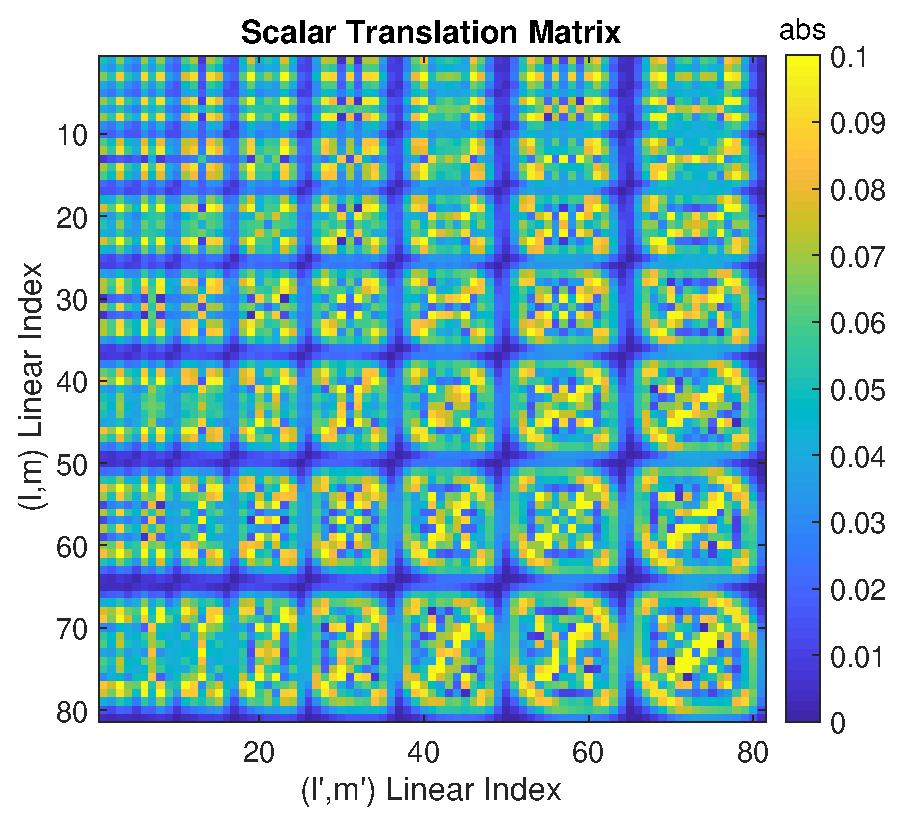
\includegraphics[width=3.5in]{Translation/Figures/transfull} 
   \caption{Scalar translation matrix, $L = L' = 8$, $k = 1$, $r_{ji} = [12, 5, 15]$.} 
\end{figure}


Adopting the notation from \cite{chew1992recurrence}, which uses the pairings $(\nu\mu,nm)$ for our $(lm,l'm')$, the recurrence relations for the full scalar translation matrix are initialized with
\eq{\alpha_{\nu\mu,00} = \sqrt{4\pi} (-1)^{\nu}Y^*_{\nu\mu}(\theta,\phi)h_{\nu}^{(1)}(k r)}

\noindent where $(r,\theta,\phi)$ are the spherical coordinates of the vector, $\br_{ji}$, that points from the originating frame to the translated frame. The first recursion relation is
\eq{b_{nn}^{+} \alpha_{\nu\mu,n+1,n+1} = b_{\nu-1,\mu-1}^{+} \alpha_{\nu-1,\mu-1,nn}  + b_{\nu+1,\mu-1}^{-} \alpha_{\nu+1,\mu-1,nn}}

This is also used to iterated on $b_{n,-n}^{+} \alpha_{\nu\mu,n+1,-(n+1)} $. The second relation is 
\eq{a_{nm}^{+} \alpha_{\nu\mu,n+1,m}  = -a_{nm}^{-} \alpha_{\nu\mu,n-1,m} + a_{\nu-1,\mu}^{+} \alpha_{\nu-1,\mu,nm} + a_{\nu+1,\mu}^{-} \alpha_{\nu+1,\mu,nm} }

The coefficients are 
\ea{a_{nm}^{+} &=& -\sqrt{ \dfrac{(n+m+1)(n-m+1)}{(2 n+1)(2 n+3)}} \\
a_{nm}^{-} &=& \sqrt{\dfrac{(n+m)(n-m)}{(2n+1)(2n-1)}} }
\ea{b_{nm}^{+} &=& \sqrt{\dfrac{(n+m+2)(n+m+1)}{(2n+1)(2n+3)}} \\
b_{nm}^{-} &=& \sqrt{\dfrac{(n-m)(n-m-1)}{(2n+1)(2n-1)} }}
Like the axial translation matrix, the computation requires a triangular fill region. As before, the fill region is placed along the dimension of the matrix with the highest degree harmonic, because we only need to fill to the smaller of $L$ and $L'$. We always fill along rows, so if the matrix needs to be flipped, the following transpose relation is used
\eq{\alpha_{mn,\nu\mu} = (-1)^{\nu+\mu+m+n} \alpha_{\nu,-\mu,n,-m}}
   
The routine \texttt{alpha} computes the full scalar translation matrix using the recursion relations above.  It takes as input the largest row degree, $L$, the largest column degree $L'$, wavenumber $k$, axial translation vector $\br_{ji}$, and returns the translation matrix linearly indexed along rows and columns. Use string switch \texttt{'rg'} for the regular form. The computation fills along rows for the larger of $L$ and $L'$, then transposes the matrix if necessary. This routine matches the outputs of the diagonalized version to machine precision. 


{\footnotesize
\VerbatimInput{\code/Translation/alpha.m}
}



\clearpage
\newpage

\section{Vector Translation Matrix}

This section gives routines for the vector axial translation matrix, sparse vector axial translation matrix, and an implementation of the diagonalized matrix-vector multiplication.  
\vspace{-1mm}
\subsection{Vector Axial Translation Matrix}

The vector axial translation matrices are found directly from the scalar axial translation matrix with the following relations:
\begin{eqnarray}
A_{l,m,l',m} &=& k r_{ji}\left[\dfrac{1}{(l+1)}\sqrt{\dfrac{(l+m+1)(l-m+1)}{(2l+3)(2l+1)}} \alpha_{l+1,m,l',m} \right. \nonumber \\
\ & \ & + \left. \dfrac{1}{l}\sqrt{\dfrac{(l+m)(l-m)}{(2l+1)(2l-1)}}\alpha_{l-1,m,l',m} \right] + \alpha_{l,m,l',m} \\
B_{l,m,l',m} &=& \dfrac{imkr_{ji}}{l(l+1)}\alpha_{l,m,l',m} 
\end{eqnarray}
\begin{equation}
A_{l,m,l',m'} = B_{l,m,l',m'} = \alpha_{l,m,l',m'} = 0, \quad \quad m \ne m'
\end{equation}

Because the first equation uses $l+1$, the scalar axial matrix needs one extra degree $l = L+1$.  The equations in \cite{mackowski1991analysis} appear to be missing several scaling factors, but \cite{chew1993efficient} gives correct equations.  Both \cite{mackowski1991analysis, chew1993efficient} derived translation matrices for partially normalized vector spherical waves functions.  For fully normalized vector spherical wave functions, the vector translation matrices need to be modified as 
\begin{eqnarray}
\widetilde{A}_{l,m,l',m'} &=& \sqrt{\dfrac{l(l+1)}{l'(l'+1)}} A_{l,m,l',m'}\\
\widetilde{B}_{l,m,l',m'} &=& \sqrt{\dfrac{l(l+1)}{l'(l'+1)}}B_{l,m,l',m'}
\end{eqnarray}

The routine \texttt{AzBz} takes as input the maximum harmonic degrees $L$ and $L'$, wavenumber $k$, and magnitude of the z-axis translation, $r_{ji}$, and returns vector translation matrices $A_{l,m,l',m}$ and $B_{l,m,l',m}$. Use string switch \texttt{'rg'} for the regular form of the matrices, and \texttt{'norm'} for fully normalized vector wave functions. 

{\footnotesize
\VerbatimInput{\code/Translation/AzBz.m}
}




\subsection{Sparse Vector Axial Translation Matrix}

Because the vector axial translation matrices are computed directly from the scalar functions, they are sparse and can be computed on a 1D array.  We only need to count the number of elements in the vector axial translation matrix and determine its sparse linear index. The number of elements in the sparse vector axial translation matrix is counted the same as the scalar case starting at $l=1$ and $l'=1$.  
\begin{eqnarray}
N(L,L') &=& \sum_{l' = 1}^{L'} \sum_{l=1}^{L} \sum_{m = -\textrm{min}(l,l')}^{\textrm{min}(l,l')} 1 \label{eq:NLL}\\
\ & = & \sum_{l' = 1}^{L'} \sum_{l=1}^{L} \left[ 2 \textrm{min}(l,l') + 1 \right]
\end{eqnarray}  

Plugging this into Wolfram Alpha
\begin{equation}
N(L,L') 
= \left\{
\begin{array}{ccc}
3 & \ & L =  L' = 1 \\
3L &\ & L' = 1, L >1\\
3L' & \ & L = 1 , L' >1\\
- 1/3L'^3  + L L'^2 + 2 LL' + 1/3L' & \ & L > 1, L' > 1, L > L'\\
-1/3L^3  + L'L^2 + 2L'L + 1/3L& \ &  L > 1, L' > 1, L'>L \\
L^2 + 5L + 2/3L'^3 + L'^2 - 14/3L' & \ & L > 1, L' > 1, L = L' \\
\end{array}
\right.
\end{equation}

Counting row-major, the sparse linear index is 
\begin{equation}
I(l,l',m,L') = N(l-1,L') + \sum_{i = 1}^{l'-1}  (2\textrm{min}(l,i) + 1)  + (\textrm{min}(l,l') + m + 1)  
\end{equation}

\noindent where
\begin{equation}
\sum_{i = 1}^{l'-1}  (2\textrm{min}(l,i) + 1) = 
\left\{\begin{array}{ccc} 
3 & \ & l + 1 \ge l' \land ((l=1 \land l' \ge 2) \lor (l' = 2 \land l > 1 )) \\
2l(l'-2) + l' + 1 & \ & l + 1 < l' \land ((l=1 \land l' \ge 2) \lor (l' = 2 \land l > 1 )) \\
l'^2 - 1  & \ & l > 1 \land l+1 \ge l' \land l > 2 \\
-l^2 + l + (2l + 1)(l'-1)& \ & \textrm{otherwise} \\
\end{array}
\right\}
\end{equation}  


The routine \texttt{AzBzSparse} returns four column arrays of the row index, column index, and matrix entries of the sparse axial translation matrices.  It is the same as \texttt{AzBz} but computed and output on a 1D array.  The helper functions are \texttt{NAzBz.m} and \texttt{indAzBz.m}.


{\scriptsize
\VerbatimInput{\code/Translation/AzBzSparse.m}
}

{\scriptsize
\VerbatimInput{\code/Translation/NAzBz.m}
}

{\scriptsize
\VerbatimInput{\code/Translation/indAzBz.m}
}

\clearpage
\subsection{Diagonalized Vector Translation Matrix}


The routine \texttt{vectorTranslation} takes as input a vector of expansion coefficients in frame $i$, $\bb{a}$ and $\bb{b}$, the maximum degrees $L$ and $L'$ of the translation matrix and the translation vector $\br_{ji}$ in Cartesian coordinates and returns expansion coefficients in frame $j$, $\bb{c}$ and $\bb{d}$. The lengths of $\bb{a}$ and $\bb{b}$ should be $L'^2 + 2L' $.  Use \texttt{'rg'} for the regular form and \texttt{'norm'} for fully normalized vector wave functions. This uses the routines for the sparse versions of the rotation matrix and axial translation matrices to save memory.  If the pair of matrices is desired, then include the optional third and fourth outputs. 


{\scriptsize
\VerbatimInput{\code/Translation/vectorTranslation.m}
}
\clearpage

\subsection{Full Vector Translation Matrix}

Like the full scalar translation matrix, recursion relations to compute the full vector translation matrices were derived in \cite{chew1993efficient}. Two versions are available: the first iterates on the vector matrices from scratch, the second iterates on the full scalar translation matrix. We implement the second version, which requires computing the scalar translation matrix at a maximum harmonic degree one higher than that of the vector matrices. 


\begin{figure}[H] 
   \centering
   \subfigure{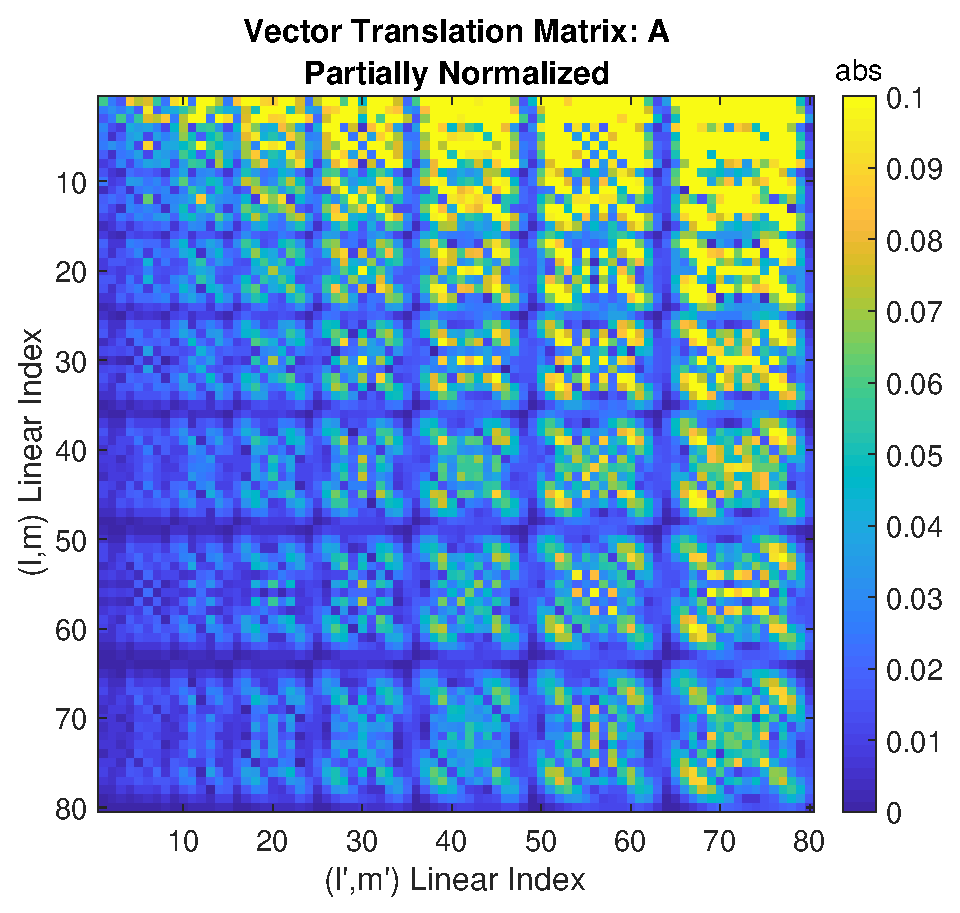
\includegraphics[width=3in]{Translation/Figures/transfullA1}}
   \subfigure{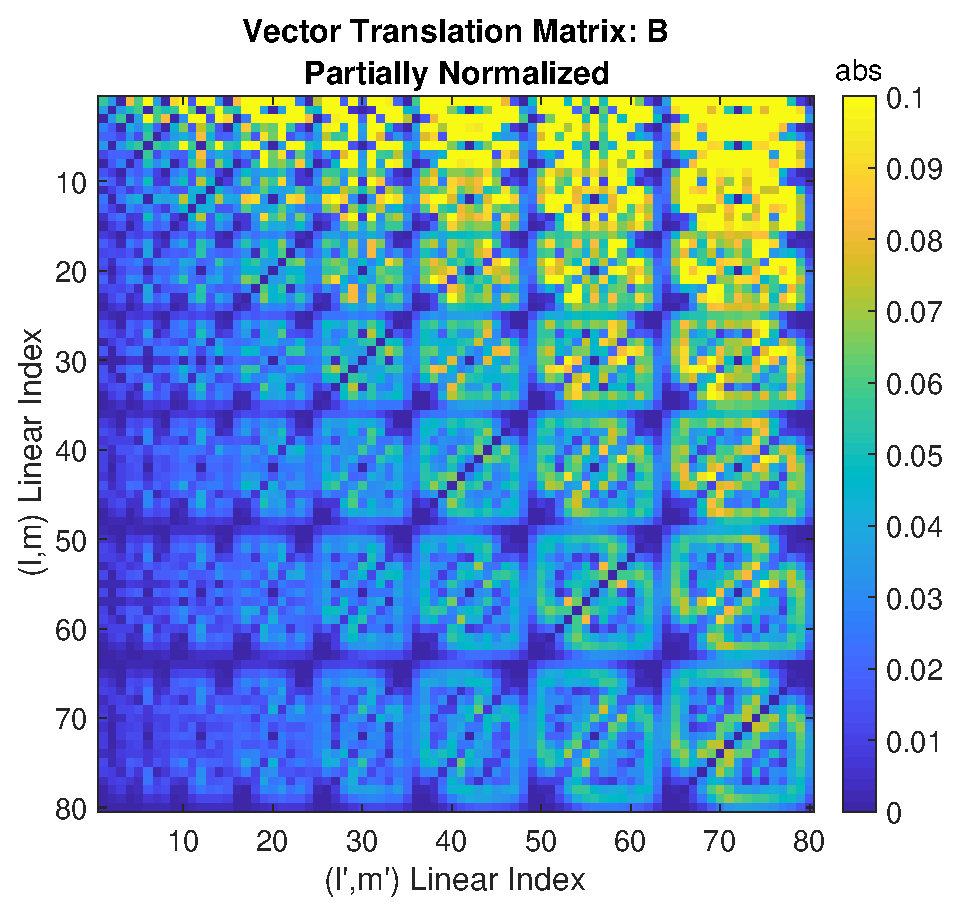
\includegraphics[width=3in]{Translation/Figures/transfullB1}} \\
   \subfigure{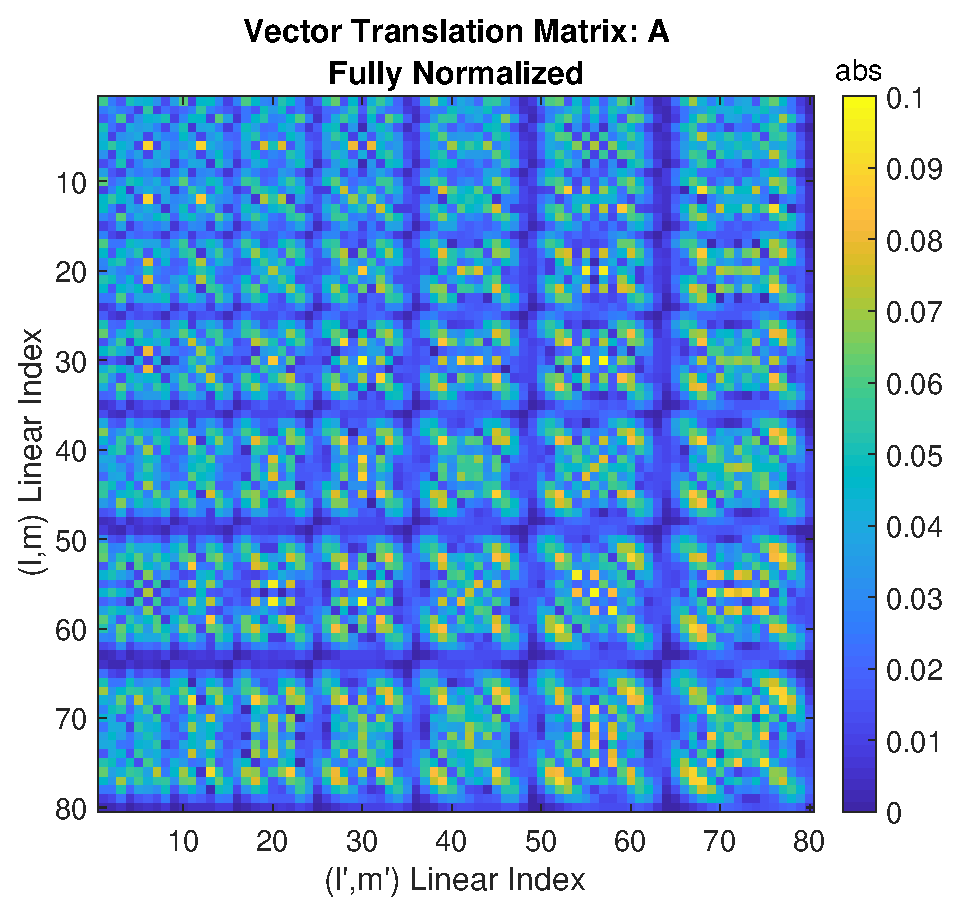
\includegraphics[width=3in]{Translation/Figures/transfullA2}}
   \subfigure{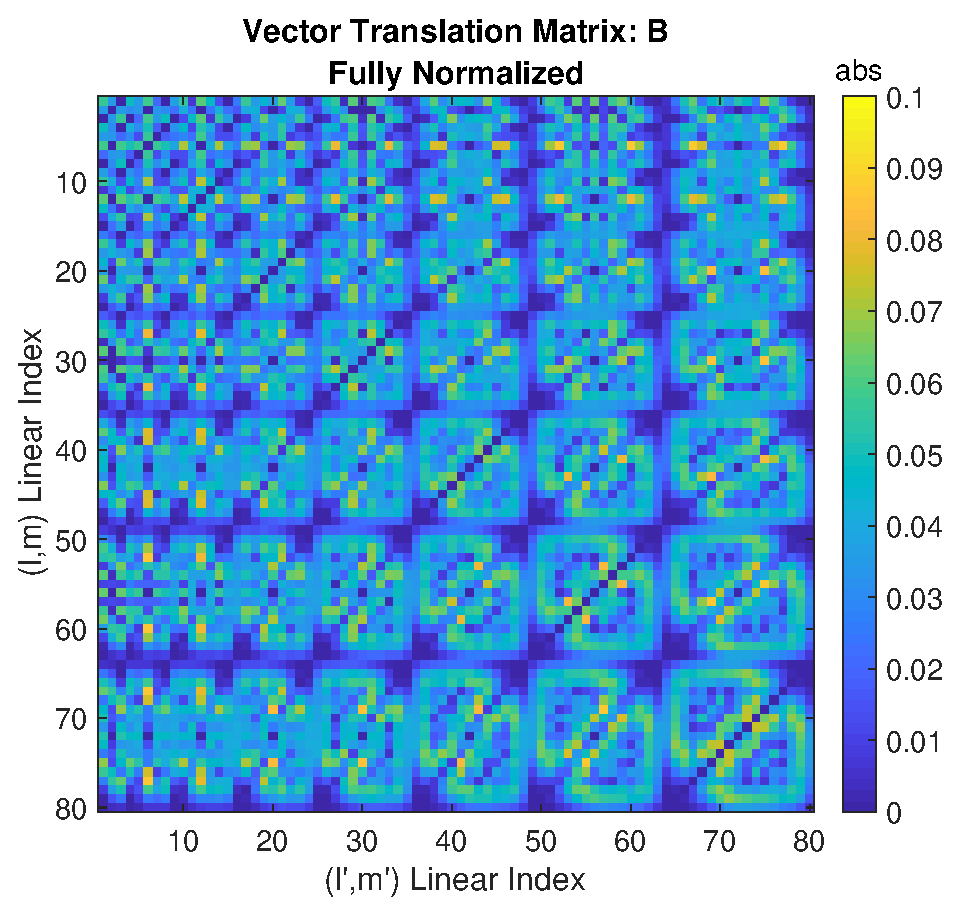
\includegraphics[width=3in]{Translation/Figures/transfullB2}}
   \caption{Vector translation matrices for $L = L' = 8$, $k = 1$, $r_{ji} = [12, 5, 15]$. Top row: matrices for partially normalized vector wave functions. Bottom row: matrices for fully normalized vector wave functions.}
   \label{transfullAB}
\end{figure}


Adopting the notation from \cite{chew1993efficient}, which uses the pairings $(\nu\mu,nm)$ for our $(lm,l'm')$, the recurrence relations for the two vector translation matrices derived from the scalar translation matrix are
\ea{A_{\nu\mu,nm} &=& \alpha_{\nu\mu,nm} + 
c_{1,\nu\mu} \alpha_{\nu+1,\mu-1,nm} + 
c_{2,\nu\mu} \alpha_{\nu-1,\mu-1,nm} + 
c_{3,\nu\mu} \alpha_{\nu+1,\mu+1,nm} + \nonumber \\
\ & \ & 
c_{4,\nu\mu} \alpha_{\nu-1,\mu+1,nm} + 
c_{5,\nu\mu} \alpha_{\nu+1,\mu,nm} + 
c_{6,\nu\mu} \alpha_{\nu-1,\mu,nm} 
\label{Anumu} \\
B_{\nu\mu,nm} &=& c_{7,\nu\mu} \alpha_{\nu\mu,nm} + 
c_{8,\nu\mu} \alpha_{\nu,\mu+1,nm} + 
c_{9,\nu\mu} \alpha_{\nu,\mu-1,nm} \label{Bnumu} } 

Note, \eqref{Anumu} and \eqref{Bnumu} only operate on the row indices $(\nu,\mu)$. The coefficients are 
\ea{
c_{1,\nu\mu} &=& \dfrac{kr\sin\theta e^{-i\phi}}{2(\nu + 1)}\sqrt{\dfrac{(\nu-\mu+2)(\nu-\mu+1)}{(2\nu + 1)(2\nu + 3)}} \\
c_{2,\nu\mu} &=&  -\dfrac{kr\sin\theta e^{-i\phi}}{2\nu}\sqrt{\dfrac{(\nu+\mu-1)(\nu+\mu)}{(2\nu - 1)(2\nu + 1)}} \\
c_{3,\nu\mu} &=& -\dfrac{kr\sin\theta e^{i\phi}}{2(\nu + 1)}\sqrt{\dfrac{(\nu+\mu+2)(\nu+\mu+1)}{(2\nu + 1)(2\nu + 3)}} \\
c_{4,\nu\mu} &=&  \dfrac{kr\sin\theta e^{i\phi}}{2\nu}\sqrt{\dfrac{(\nu-\mu)(\nu-\mu-1)}{(2\nu - 1)(2\nu + 1)}}\\
c_{5,\nu\mu} &=& \dfrac{kr\cos\theta}{\nu+1}\sqrt{\dfrac{(\nu+\mu+1)(\nu-\mu+1)}{(2\nu + 1)(2\nu + 3)}} \\
c_{6,\nu\mu} &=&  \dfrac{kr\cos\theta}{\nu}\sqrt{\dfrac{(\nu+\mu)(\nu-\mu)}{(2\nu - 1)(2\nu + 1)}}  \\
c_{7,\nu\mu} &=& \dfrac{i\mu kr\cos\theta }{\nu(\nu+1)} \\
c_{8,\nu\mu} &=& \dfrac{i kr\sin\theta e^{i\phi} }{2\nu(\nu+1)} \sqrt{(\nu-\mu)(\nu+\mu+1)} \\
c_{9,\nu\mu} &=& \dfrac{i kr\sin\theta e^{-i\phi} }{2\nu(\nu+1)} \sqrt{(\nu+\mu)(\nu-\mu+1)}  } 

\noindent where $(r,\theta,\phi)$ are the spherical coordinates of the vector $\br_{ji}$ that points from the originating frame to the translated frame.


The routine \texttt{AB} takes as input the maximum harmonic degrees $L$ and $L'$, wavenumber $k$, and translation vector, $r_{ji}$, and returns full vector translation matrices $A$ and $B$. It calls \texttt{alpha} to compute the full scalar translation matrix. Use string switch \texttt{'rg'} for the regular form of the matrices, and \texttt{'norm'} for fully normalized vector wave functions. 



{\footnotesize
\VerbatimInput{\code/Translation/AB.m}
}




